\begin{document}
\chapter{Procesarea de imagini pe dispozitive mobile}
	Dispozitivele mobile au avut o evolutie constantă pe parcursul timpului. În ziua de astăzi multe dintre aceste dispozitive mobile ating perfomanțe mult mai ridicate decat ale unor laptopuri cu o vechime de 10 ani. 
	Deși dispozitivele mobile sunt perfecte pentru realizarea unor activități de zi cu zi si sunt capabile să facă față unor aplicații costisitoare din punctul de vedere al complexității, forța lor de computație este relativ slabă, în comparație cu cea a calculatoarelor și a laptopurilor. Dispozitivele mobile nu profită de aceeasi cantitate de memorie CPU și GPU de care profită calculatoarele și laptopurile, rezultând intr-o perioadă de timp prelungită necesară pentru finalizarea antrenării unui model de rețele neuronale cu un număr mare de filtre, straturi si operații, cum ar fi augmentarea datelor.
	
	\section{Istoria dispozitivelor mobile}
	Ideea telefoanelor fără fir a apărut încă din perioada primului razboi mondial, când armata germană testa comunicarea independentă de fir în interioriul trenurilor militare. Dezvoltarea acestor dispozitive de comunicare a luat amploare foarte repede. In jurul anului 1940, în perioada celui de al doilea razboi mondial, emițîtoarele radio portabile jucau un rol crucial in comunicarea armatei.
	Tehnologia de comunicare prin emițătoare radio folosită de armată, a inspirat mai departe compania de cercetare științifcă Bell Labs in crearea dispozitivelor dependente de mașină, în anul 1946. Prin intermediul acestor dispozitive devenea posibilă comunicarea telefonică din interiorul mașinilor (vezi Fig. \ref{fig:tanti-telefon}).
	
	\begin{figure}[H]
		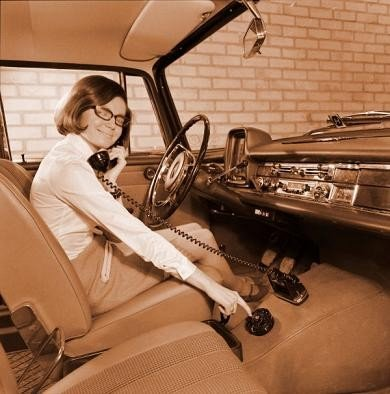
\includegraphics[width=10cm]{tanti-telefon}  
		\caption{\label{fig:tanti-telefon} Telefonul de mașină creat de Bell Labs
			\protect
			\cite{phone_lady}}
	\end{figure}
	

	La scurt timp după inovația adusă de către Bell Labs, AT\char`&T, compania americană specializată în telecomunicații, va avea să ofere servicii de telefonie mobilă si canale de comunicare pe zone restrânse. Dispozitivul oferit de către AT\char`&T era asemănător un transmițător radio. Era necesară apăsarea unui buton pentru a putea transmite un mesaj vocal, iar pentru a asculta interlocutorul, era necesară eliberarea butonului. Pentru a putea utiliza serviciile oferite de AT\char`&T in mașină, era nevoie de atașarea unui echipament care cântărea aproximativ 36 de kg.
	In 1949, serviciul telefonic susținut de AT\char`&T găzduia în jur de  5,000 de utilizatori, care realizau săptămânal aproximativ 30,000 de apeluri telefonice. Toate aceste apeluri telefonice erau gestionate manual de către operatori ai companiei AT\char`&T. 
	
	Un serviciu asemănător celui oferit de AT\char`&T, a fost creat în Regatul Unit și se numea Post Office Radiophone Service. Diferența facută de acest serviciu telefonic a fost modul în care erau gestionate apeluri telefonice. Deși erau gestionate in continuare de un operator, un apel telefonic putea fi realizat între oricare doi participanți din intregul Regat Unit. 
	
	Serviciul a fost creat în Manchester in 1959, adus in Londra in 1965, după care a fost distribuit in 1972 celorlalte orașe mari din Anglia.
	În anul 1983 va avea să apară primele telefoane mobile ce puteau fi tinute în mână. Primul producător de telefoane mobile a fost Motorola iar primul model a fost Motorola DynaTAC 8000x (vezi Fig.\ref{fig:dynatac}). Prețul său creștea până la 4000 de dolari, fiind un dispozitiv voluminos și greu (cântărind în jur de 4 kg)  având o baterie capabilă de a susține 30 de minute de convorbire. În ciuda dimenisiunii mari a acestuia, era considerat cea mai bună variantă din punctul de vedere al portabilității datorită faptului ca va avea să pună capăt dependenței cablurilor telefonice pentru a purta o convorbire.

	
	În anii 1990 au inceput să apară telefoane mobile aparținând generației a doua de dispozitive mobile. Acestea utilizau transmisie digitală, tehnologie ce aducea un plus de securitate și viteză peste transmisia analog. Odata cu această generație de dispozitive mobile, apar și SMS-urile (Short Message Service), prima utilizare fiind in 1993.
	În 1993, deși o teorie controversată, apare primul smartphone. IBM lansează modelul Simon. Acesta dispunea de: ceas, calendar, agenda telefonică, notițe, căsuță de email, auto-completare si touchscreen. (vezi Fig. \ref{fig:simon})
	
	
	
	\begin{figure}[H]
		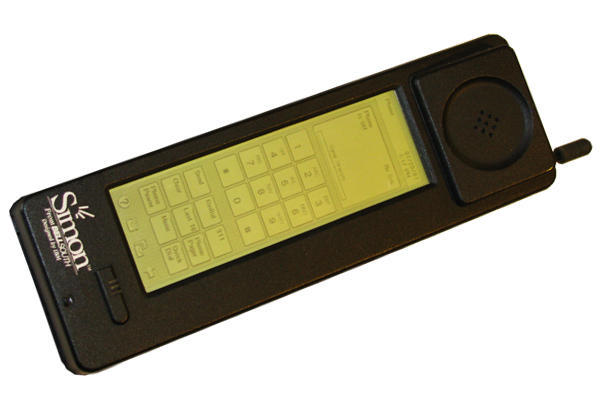
\includegraphics[width=8cm]{simon}  
		\caption{\label{fig:simon} Modelul de celular IBM Simon
			\protect
			\cite{ibm_simon}}
	\end{figure}
	
	
	După apariția modelului Simon, creat de IBM, dispozitivele mobile vor avea să urmeze un progres remarcabil în termen de funcționalitate, stil și cel mai important, forță de computație. 
	Telefoanele mobile au reușit să introducă în buzunarul oamenilor forța de procesare, de la utilizarea unui simplu serviciu de email sau calendar, până la utilizarea aplicațiilor ce dispun de inteligență artificiala. \cite{history_cellphones}
	\newline
	
	\section{Arhitecturi ARM}
	Pe parcursul timpului, calculatoarele și dispozitivele mobile au întâlnit mai multe arhitecturi ce au stat la baza componentei lor de baza, CPU. Acestea au fost dezvoltate ținând cont de necesitatea de computație de care are nevoie un sistem de calcul. Astăzi se pot enumera trei mari arhitecturi prezente in majoritatea dispozitivelor: arhitectura Intel x86, respectiv x86\char`_64 și arhitectura ARM. 
	
	Diferența între cele două mari tipuri de procesoare o face modul în care acestea gestionează computația. Procesoarele cu arhitectură Intel x86 și x86\char`_64 sunt bazate pe arhitecturi CISC (Complex instruction set computing) ce prezintă computație complexă, concentrată si plasată pe un număr relativ mic de nuclee. Acest lucru aduce avantajul forței mari de computație și multe operații per ciclu, însa crește proporțional consumul de energie. În contrast, procesoarele ARM sunt dezvoltate peste arhitectura RISC (Reduced Instruction Set Computing), care sunt reprezentate prin mai multe operații simple și scurte, rezultând în mai puține operații per ciclu dar și consum relativ redus de energie. 
	
	Neajunsurile arhitecturii de tip x86 sunt in continuare duse mai departe de calculatoarele cu sistem de operare Windows datorită compatibilității între versiuni, un factor important de care Microsoft ține cont. Acest lucru face pe moment imposibilă trecerea de la arhitecturi de tip x86 si x86\char`_64 spre arhitecturii ARM. 
	
	Deoarece dispozitivele mobile fiind relativ noi nu depind de arhitectura x86 și au putut fi dezvoltate peste arhitecturi ARM. Acest lucru este un factor important, datorită costului redus de energie pe care procesoarele ARM îl exercită. Datorită circuitelor mult mai scurte și a necesităților reduse la nivel de computatie datorate numărului mic de tranzistori, acestea sunt de altfel reduse in dimensiune, aducând un plus in utilizarea lor ca și componenta a dispozitivelor mobile.
	
	Arhitecturile de tip ARM nu sunt noi. Acestea sunt prezente încă din anul 1980, aduse pe piață de compania Acorn RISC Machines Ltd. iar abrevierea provine de la Advanced RISC Machines. 
	
	Un avantaj important al arhitecturii ARM este posibilitatea de scalabilitate. Dat fiind raportul relativ îmbunătățit de performanță per watt, aplicațiile pot utiliza mai multe nuclee simple ale plăcii ARM si pot beneficia de consumul redus de energie. În timp ce procesoarele 
	Intel X86 realizează operatii complexe pe un număr redus de nuclee puternice computațional, procesoarele ARM pot împărți într-un număr mult mai mare de nuclee. Acest lucru devine optim în cazul unei aplicații software dezvoltată tinând cont de această modularizare si scalabilitate.
	\cite{arm_architecture_android}
	
	Lupta imbunatatirii capabilitatii procesoarelor si componentelor hardware ale telefonului mobile, sunt duse in scopul portarii operatiilor de inferenta a retelelor neuronale complexe (Deep Neural Networks) de pe cloud chiar pe dispozitivul celular, in scopul diminuarii timpului obtinut pe parcursul etapei de transfer de date (TCP/IP si protocoale aferente). Avansarea componentelor de tip hardware aduc un plus doar de moment, urmand a-si pierde de eficienta in timp. Pentru a obtine o optimizare buna a serviciilor de inferenta, trebuiesc luate in calcul diferite metode de accelerare a operatiilor. Incepand de la arhitecturi scalabile si ne-consumatoare ARM, abstractizarea operatiilor responsabile de hardware si expunerea unei interfete pentru utilizarea acestora eficient si pana la optimizarea unor algoritmii in scopul sprijinirii arhitecturilor reduse in puterea de computatie.
	
	Accelerarea inferentei retelelor neuronale este un obiectiv luat in calcul in momentul actual de multe dintre companiilor producatoare de dispozitive mobile. Apple vine, incepand cu modelul Iphone X, cu acceleratorul Neural Engine, specializat pe operatiile inferentei, iar Microsoft HoloLens vin cu HPU CNN. \cite{arm_ml}
	
	\section{Sistemul de operare Android}
	
	Android este un sistem de operare Open Source dezvoltat si intretinut de catre compania Google. Google a cumparat in anul 2005 compania Android Inc., o companie ce se ocupa cu sisteme de operare pentru camere foto digitale si telfoane mobile, cu scopul intrarii pe piata dispozitivelor mobile. Dupa 2 ani de la cumpararea companiei, Google lanseaza sistemul de operare pe piata. 
	
	In momentul de fata, 85\% din totalitatea utilizatorilor dispozitivelor mobile smartphone, utlizeaza sistemul de operare Android. 
	
	Ceea ce face sistemul de operare Android, un punct de interes in viziunea invatarii automate, este arhitectura sa. Android are la baza o versiune a nucleului Linux, sistem de operare care face parte din familia UNIX. Sistemul de operare poate rula pe arhitecturi ARM. 
	
	Incepand din anul 2012, dispozitivele mobile Android sunt dezvoltate utliziand procesoare Intel iar mai tarziu se vor stabili pe arhitecturi de 64-bit, ARM64. 
	Forta pe care procesoarele dispozitivelor mobile o aduc, impreuna cu sistemul de operare Android, ne permit utilizarea multor tehnici de invatare automata chiar pe sistemul telefonului. 
	
	Desi placa de baza a dispozitivelor mobile permite rularea unor computatii complexe si utilizarea procesurilor si a firelor de executii, acestea permit de altfel utilizarea placii grafice (GPU), in scopul realizarii unor computatii intense distribuite.
	
	\subsection{Android System Developer Kit}
	
	Android System Developer Kit, sau Android SDK, este interfata expusa de Google, in scopul dezvoltarii de aplicatii si widgeturi pentru dispozitivele mobile Android, aparuta in 2008. Android SDK este un tool ce face  functionalitatile de baza ale telefonului mobil (cum ar fi camera, miscrofonul sau giroscopul) usor de utilizat, ofera biblioteci programabile, conditii de compilare, depanare si emulare a modelelor de dispozitive Android. 
	Sistemul de operare poate fi impartit in 5 componente:
	\begin{itemize}
		\item Aplications. Acestea sunt produsele finale la care au acces utilizatorii.
		
		
		\item Application Framework. Application Framework este baza programabila care usureaza utilizarea unor functionalitati precum: camera video sau foto, activitati, servicii de messaging, etc.
		
		\item Libraries. Penru a usura utilizarea bazelor de date, Secure Socket Layer, OpenGL, etc., au fost aduse la indemana programatorilor, biblioteci specializate in utilizarea acestor tehnologii.
		
		\item Android Runtime. Aplicatiile au nevoie de o masina virtuala pentru a rula. Android Runtime contine toate rutinele necesare pentru a compila si a rula o aplicatie.
		
		\item Linux Kernel. Pentru a accesa componentele hardware ale telefonului, sistemul de operare foloseste interefete numite "drivers". Acestea sunt rutine ce opereaza low-level cu placa de baza.
	\end{itemize}
	
	\vfill
	
	Pe parcursul dezvoltarii proiectului Android, acesta a trecut prin diferite versiuni, fiecare aducand o extensie in materie de functionalitati si imbunatatiri soft sistemului de operare. Desi proiectul era orientat spre progres, dezvoltarea s-a facut tinand cont de compatibilitatea anterioara. Astfel, versiunile noi ale sistemului de operare, pot rula aplicatii cu o vechime mai mare decat acestea.
	
	Prima versiune de Android a fost Astro 1.0. Aceasta rula pe modelul HTC Dream si detinea multe dintre aplicatiile care sunt inca utilizate in ziua de astazi. Printre aceste aplicatii se numara Android Market, Gmail, Google Maps etc.
	La aprope doi ani dupa aparitia versiunii Astro, apare versiunea 1.5 Cupcake. Aceasta rula pe un nucleu Linux 2.6, si a adus multe avantaje utilizatorilor si programatorilor. Aceasta versiune a introdus widgeturi, animatii si alte functionalitati la nivelul dispozitivelor cu Bluetooth.
	\newline
	
	Pe parcursul dezvoltarii, fiecare versiune aparuta a adus o imbunatatire in materie de funtionalitate sau interfata vizuala, insa un punct critic in dezvoltarea sistemului de operare si unul memorabil pentru invatarea automata, a fost versiunea 4.0, Ice Cream Sandwich. Aceasta versiunea a fost lansata in anul 2011 si este bazata pe un nucleu Linux, versiunea 3.0. Pe langa imbunatatirile aduse interfatei vizuale si flexibilitatii de configurare, versiunea Ice Cream Sandwich introduce utilizarea algoritmilor inteligenti de detectare a fetei si posibilitatea de a debloca telefonul utilizand recunoastere faciala. 	
	Acest punct marcheaza posibilitatea utilizarii algoritmilor de invatare automata pe dispozitivele mobile, fiind un imbold spre avansarea invatarii automate pe acest plan. Dezvoltarea proiectului a tinut cont din acest moment, de necesitatea utilizarea algoritmilor inteligenti pe dispozitive mobile, astfel s-a pus accent pe accelerarea hardware si minimalizarea costului sistemelor inteligente. Avansarea componentelor hardware nu constituie intregul motiv pentru care utilizarea algoritmilor inteligenti a devenit posibila, ci si simplificarea si optimizarea acestora pentru a fi utilizati in parametri optimi de rulare.
	\newline
	
	Desi exista alternative pentru dezvoltarea de aplicatii pe dispozitive Android, interfata oferita de Google este cea mai populara ca si numar de utilizatori. Un aspect important al acestei interfete, este flexibilitatea pe care o ofera, in materie de limbaje de programare. Aplicatiile Android pot fi dezvoltate pe baza Android SDK, utilizand limbajele de programare Java, C++ si Kotlin. \cite{android}	
	Android SDK expune modalitati de a procesa imaginile preluate din camera video a dispozitivului. Aceste modalitati, impreuna cu bilblioteci specializate in computatii distribuite utilizand forta GPU, ne permite utilizarea unor algoritm de invatare automata. 
	
	Android introduce in versiunea API 21, o versiune noua a interfetei programabile ce gestioneaza camera video a dispozitivului mobil, Camera 2 API. Aceasta interfata acopera utilizarea camerei, de la permisiune pana la selectarea unei camere dintr-o lista de dispozitive disponibile si procesarea in mod continuu a imaginilor captate.
	
	
\end{document}